\chapter[Referencial teórico]{Referencial teórico}\label{ch:referencial}

(a fazer)
(- dividir em macro-seções)
(- cadenciar uma seção para a outra melhorando a leitura)
(- ligar os termos ao tema)
(- considerações finais do capítulo)
\cite{serrano2011}
\cite{jennings2000}
\cite{zambonelli2001}

\section{Agentes}

Existem diferentes definições para agentes. Ainda assim, estas definições possuem conceitos básicos em comum como sugere \citeonline{mcarthur2007multi}: a noção de agente, seu ambiente e sua autonomia. Para o autor e para \citeonline{jennings1996}, um definição flexivel para agentes é que são entidades de software ou hardware capazes de reagir e tomar decisões de forma autônoma, com base nas alterações do ambiente o qual está situado. \citeonline{selker1994} destaca que agentes são softwares que simulam uma relação humana, realizando tarefas que poderiam ser executadas por pessoas.

Agentes podem ser representados por seis características ortogonais conforme ilustrado na Figura \ref{fig:hexagono}: adaptabilidade, autonomia, inteligência, mobilidade, persistência e cooperação. Tais características, atuando em conjunto, tornam o agente mais robusto e suscetível a mudanças \cite{griss2001software}. Quanto maior for a área fechada no diagrama, mais aquele componente do sistema pode ser classificao como agente \cite{griss2001software}.

\begin{figure}[h!]
    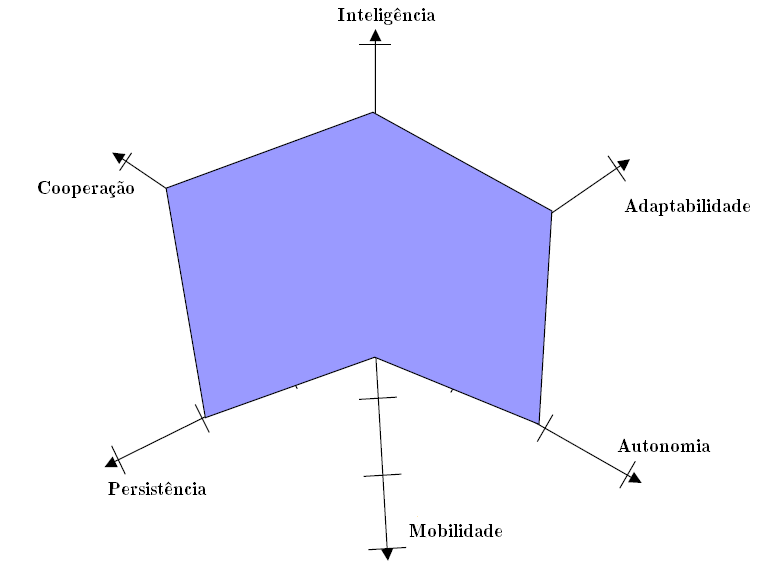
\includegraphics[scale=0.6]{figuras/hexagono_agente}
    \centering
    \caption{Dimensões do agente. Fonte: \cite{griss2001software}. Traduzido.}
    \label{fig:hexagono}
\end{figure}

Um agente pode ter seu comportamento alterado após sua implantação, o grau com que isto é possível denomina-se adaptabilidade. A autonomia de um agente, por sua vez, é definida como o grau com que é responsável pelo controle da sua própria \textit{thread} e o grau com que pode prosseguir em sua meta individual independentemente de mensagens enviadas de outros agentes \cite{griss2001software}.

O agente também se caracteriza por sua capacidade de raciocinar sobre suas metas e seus conhecimentos. O grau com que o agente possui esta capacidade denomina-se por inteligência. Conjuntamene, agentes possuem mobilidade, que se trata da habilidade de um agente passar da execução de contexto para outro. Ou seja, o agente pode continuar sua execução em um novo contexto enquanto mantém seu estado \cite{griss2001software}.

A infra-estrutura oferecida aos agentes pode permitir que conservem tanto conhecimentos adquiridos quanto seu estado durante longos períodos de tempo. Pode contriBuir também para a robustez dos agentes diante de possíveis falhas em tempo de execução. O grau com que a infra-estrutura cumpre estes critérios intitula-se persistência \cite{griss2001software}.

Ademais, agentes possuem cooperação, que se trata do grau em que os agentes se comunicam e trabalham em cooperação uns com os outros para formar Sistemas Multiagentes \cite{griss2001software}. Em sentido semelhante, \citeonline{wooldridge1995} destacam outros atributos como habilidade social - a interação entre agentes através de linguagem de programação voltada para agentes -, reatividade -  diz respeito à responder em tempo hábil às mudanças que ocorrem no ambiente percebido pelo agente - e, por fim, proatividade - agentes possuem comportamento dirigido à meta, o que significa que possuem a habilidade de tomar iniciativas por conta própria.

\section{Sistemas multiagentes}

Sistemas multiagentes se enquadram no cenário onde coexistem dois ou mais agentes \cite{mcarthur2007multi}. Tais agentes se comunicam tipicamente através da troca de mensagens através da infra-estrutura de rede fornecida \cite[pág. 3]{livrao}.

\citeonline{mcarthur2007multi} ressaltam que não há um objetivo geral do sistema, mas metas locais de cada agente em separado. As intenções do projetista para o sistema só pode ser realizada através da inclusão de vários agentes inteligentes.

um agente pode descobrir por si mesmo o que ele precisa fazer a fim de satisfazer os objetivos para os quais foi projetao, ao invés de ter que lhe ser dito explicitamente o que fazer em um dado momento.

 Segundo \citeonline{livrao}, no caso mais geral, os agentes em um sistema multiagente representa ou atua em nome dos usuários ou proprietários com diferentes objetivos e motivações. Para que interajam com sucesso, tais agentes exigem a capacidade de cooperar, coordenar e negociar uns com os outros, da mesma forma que as pessoas podem cooperar, coordenar e negociar com as outras na vida cotidiana \cite[pág. 3]{livrao}.

Um agente representa e raciocina sobre os outros agentes no ambiente \cite[pág. 887]{van2008handbook}. 

um sistema multiagente é por natureza \textit{multi-thread}, em que cada agente possui pelo menos um \textit{thread} \cite[pág. 27]{livrao}.


jennings2000

Como estabelece \apudonline[pág. 42-43]{serrano2011}{jennings2000}, sistemas multiagentes possuem basicamente seis elementos: agentes, interação, organização, recursos, esfera de influência e ambiente (Figura \ref{fig:sma_estrutura}). A interação pode ocorrer entre os agentes e o meio ambiente, bem como entre os agentes por meio de protocolos específicos. A organização se situa dentro do ambiente determinando quais tarefas serão executadas pelos agentes de modo a satisfazer os usuários. 

Para que concluam suas tarefas, os agentes e a organização podem usufruir dos recursos presentes no ambiente. \apudonline[pág. 42-43]{serrano2011}{jennings2000} explica que cada elemento contém uma esfera de influência no ambiente em análise. Esta esfera representa a influência de cada elemento do ambiente, enfatizando a importância deles para alcançar com êxito os objetivos. A comunicação permite lidar com as informações trocadas entre os agentes, centrando-se na percepção e ações envolvidas neste processo interativo.

\begin{figure}[h!]
    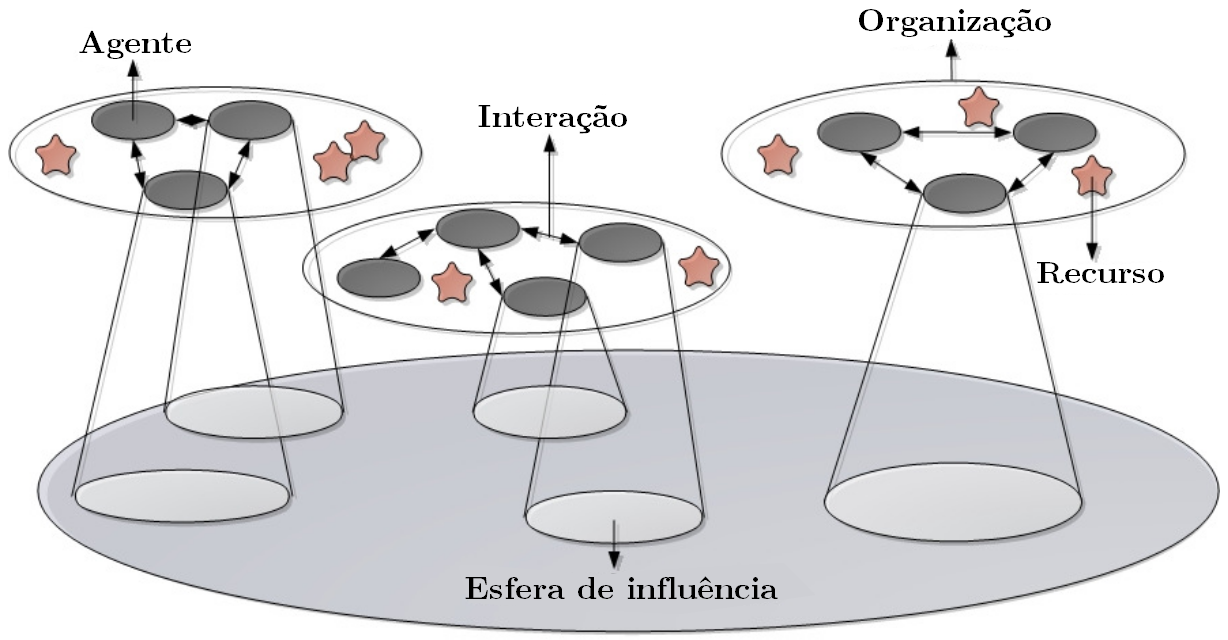
\includegraphics[scale=0.3]{figuras/sma_estrutura}
    \centering
    \caption{Estrutura de sistemas multiagentes  \apud{jennings2000}{serrano2011}}. Traduzido.
    \label{fig:sma_estrutura}
\end{figure}


\section{\textit{Framework i*}}


O framework i * propõe uma abordagem orientada a agente para a centralização de engenharia de requisitos nas características intencionais do agente. Agentes atribuem propriedades intencionais (tais como objetivos, crenças, habilidades, compromissos) entre si e raciocinam sobre relacionamentos estratégicos. Dependências entre agentes dão origem a oportunidades, bem como vulnerabilidades. Redes de dependências são analisadas utilizando uma abordagem de raciocínio qualitativo. Agentes consideram configurações alternativas de dependências para avaliar o seu posicionamento estratégico em um contexto social.

O framework é usado em contextos nos quais há múltiplas partes (ou unidades autónomas) com interesses estratégicos que podem servir de reforço ou entrar em conflito em relação ao outro. Exemplos de tais contextos incluem: redesenho de processos de negócios, redesenho de negócios, engenharia de requisitos de sistemas de informação, analisando a incorporação social da tecnologia da informação, eo projeto de sistemas de software baseados em agentes.

O nome i * (pronuncia-se por "i estrela" ou \textit{"i star"}) refere-se ao conceito de intencionalidade distribuída.

\section{Padrão}

(a fazer)

\section{Catálogo de padrões}

Um catálogo de padrões é um conjunto de padrões relacionados; por vezes vagamente ou informalmente relacionados. No catálogo, os padrões são subdividios em categorias abrangentes podendo incluir referências cruzadas entre os padrões \cite{appleton1997}. O catálogo de padrões pode incluir a apresentação da estrutura e organização do padrão, mas normalmente não apresenta algo além da estrutura e das relações mais  facilmente identificáveis \cite{appleton1997}.

A exemplo de \citeauthor{gamma1995} (\citeyear{gamma1995}), foram organizados 23 padrões de projeto orientados a objetos em um catálogo. Este catálogo descreve boas soluções de software de uso genérico, ou seja, padrões que independem do domínio de aplicação. Os autores utilizaram dois critérios para classificar os padrões de projeto: (i) escopo e (ii) propósito. Assim, pôde-se comunicar e exibir as relações entre os padrões.

Portanto, em resumo, para caracterizar um catálogo de padrões deve-se fornecer:

\begin{itemize}
    \item Categorias de padrões;
    \item Critérios de classificação do padrão (em categorias);
    \item Relacionamentos/Referências cruzadas entre padrões.
\end{itemize}



\section{Arquitetura de software}

\subsection{Componente}

De acordo com o SWEBOK \cite{swebok}, um componente de software é uma unidade independente do software. Esta unidade é compreendida em interfaces e dependências bem definidas. Corroborando com esta ideia, \citeauthor{buschmann2007} define componente como parte independente, destacável e executável de um software. Sua responsabilidade é implementar um serviço específico ou um conjunto de serviços de outros componentes ou clientes. 

Um componente provê uma ou mais interfaces que permitem o acesso aos seus serviços. Podem ser comparados a "blocos de construção" para a estruturação de um sistema. Embora um componente seja independente, componentes podem possuir dependências ou ser compostos de outros componentes. Para \citeauthor{buschmann2007} (\citeyear{buschmann2007}), os componentes podem ser representados como módulos, classes ou um conjunto de funções relacionadas. 

%%
Arquitetura é a estrutura ou organização de componentes 

\begin{citacao}
"A arquitetura de software é uma descrição dos subsistemas e componentes de um sistema de software e as relações entre eles. Subsistemas e componentes são muitas vezes especificados por meio de diferentes pontos de vista para mostrar as propriedades funcionais e não funcionais relevantes de um sistema de software. A arquitetura de um sistema de software é um artefato que resulta de atividades de projeto de software \cite{buschmann2007}."
\end{citacao}

\section{Padrão arquitetural}


\citeonline{avgeriou2005} definem padrões arquiteturais como soluções bem estabelecidas para problemas arquiteturais. Tais soluções ajudam a documentar as decisões de projeto de arquitetura, descrevem atributos de qualidade do sistema. Padrões arquiteturais facilitam a comunicação entre as partes interessadas - \textit{stakeholders} - através de um vocabulário comum.

Padrões arquiteturais são considerados como pares problema-solução que ocorrem em um determinado contexto e se afetam por ele \cite{avgeriou2005}. Além disso, um padrão não apenas indica "como" uma solução resolve um problema, mas também torna explícito o "porquê" do problema ser resolvido, ou seja, qual a lógica por trás desta solução em particular \cite{avgeriou2005}. 

A descrição dos padrões arquiteturais se baseia no tripé problema-solução-contexto.

e pode ser ainda mais elaborado com detalhes mais ricos, com especial incidência sobre a lógica por trás de uma solução. Finalmente, há uma série de postulados para uma solução para os qualificar como um padrão. Por exemplo, o padrão tem de capturar a prática comum (por exemplo ter pelo menos três utilizações conhecidas) e, ao mesmo tempo, a solução do padrão devem ser não-óbvia \cite{avgeriou2005}.

Em particular, a descrição do problema presta muita atenção para as causas que moldam o problema, enquanto a solução detalha como (e se) essas causas são resolvidas. 

Padrões podem ser usados em combinação conforme explicam \citeonline{shaw1996}, \citeonline{avgeriou2005}. Podem trabalhar em conjunto fornecendo pontos de vista complementares durante o projeto inicial ou elaborando um determinado componente de um padrão usando algum outro padrão \cite{shaw1996}. Portanto, é possível que hajam numerosas interdependências entre padrões \cite{avgeriou2005}. Estas combinações podem ocorrer repetidamente até que questões de arquitetura sejam resolvidas dando lugar às técnicas de programação convencionais \cite{shaw1996}.

No trabalho de \citeonline{shaw1996}, a descrição de cada padrão inclui notas sobre: 



\section{Arquitetura de Sistemas Multiagentes}


(a fazer)

\section{Estruturas organizacionais}

\cite{kolp2006}


\section{FIPA ACL}


